The background model uses a mixture of gaussians method, looking at all three color channels in the image. The output of the background model is a reference to a frame object containing the probability of a pixel being part of the background.

\subsubsection{Expectation maximization}
The normal expectaion maximation algortihm is too slow to run in real time, so we use a somewhat simplified version outlined in Wood (2007).

See code in appendix \ref{sec:BGMod_code}. %referens till kod, ger klickbar länk.

\begin{figure}[htb]
	\centering
	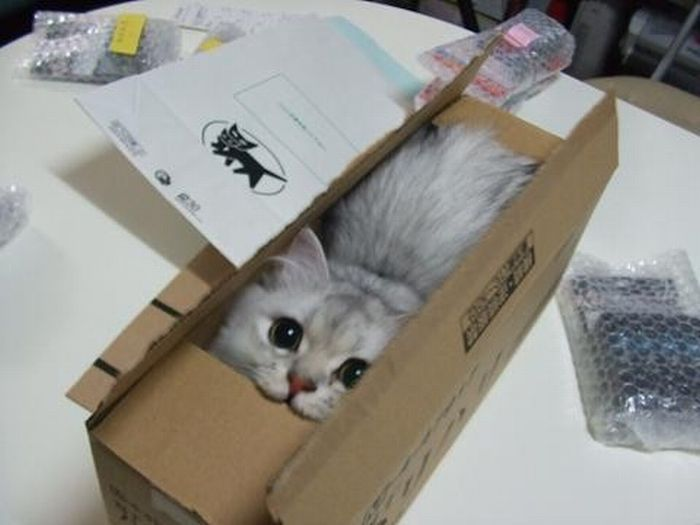
\includegraphics[width=\linewidth]{images/acatisfinetoo}
	\caption{\textit{Background modeling figure.}}
	\label{fig:BGModeling_fig} %Skapar referens till figuren
\end{figure}

\subsubsection{Solution}
A pixel that belongs to the background is static over time, as the background does not move. Each pixel is assigned a model for its variance over time, that is updated with each frame. With each frame, each pixel’s intensity is compared to the model and the deviation from the modeled intensity is the probability that the pixel belongs to an object not occluding the background.

Pixels determined to belong to the background in the previous frame will not have their probability models updated to prevent them from bleeding over into the background model.
This can be seen in figure \ref{fig:BGModeling_fig}. %Referens till figur, Ger klickbar länk i pdfen.
